\section{Scenarios Tables}

\begin{table}[!htbp] \centering 
  \caption{Ordered Size} 
  \label{} 
\begin{tabular}{@{\extracolsep{5pt}} ccccc} 
\\[-1.8ex]\hline 
\hline \\[-1.8ex] 
 & Sorting & Size.Value & LCI & UCI \\ 
\hline \\[-1.8ex] 
 & Ordered & $0.914$ & $0.912$ & $0.917$ \\ 
 & Not Ordered & $0.958$ & $0.949$ & $0.968$ \\ 
\hline \\[-1.8ex] 
\end{tabular} 
\end{table} 

\begin{table}[!htbp] \centering 
  \caption{Ordered Coverage} 
  \label{} 
\begin{tabular}{@{\extracolsep{5pt}} ccccc} 
\\[-1.8ex]\hline 
\hline \\[-1.8ex] 
 & Ordered.Unordered & Cov.Value & LCI & UCI \\ 
\hline \\[-1.8ex] 
 & Ordered & $0.998$ & $0.997$ & $1.000$ \\ 
 & Not Ordered & $0.958$ & $0.949$ & $0.968$ \\ 
\hline \\[-1.8ex] 
\end{tabular} 
\end{table} 

\begin{table}[!htbp] \centering 
  \caption{OR Size} 
  \label{} 
\begin{tabular}{@{\extracolsep{5pt}} cccccc} 
\\[-1.8ex]\hline 
\hline \\[-1.8ex] 
 & Ordered.Unordered & OR & Size.Value & LCI & UCI \\ 
\hline \\[-1.8ex] 
1 & Not Ordered & $1.050$ & $0.910$ & $0.909$ & $0.910$ \\ 
2 & Not Ordered & $1.100$ & $0.910$ & $0.909$ & $0.911$ \\ 
3 & Not Ordered & $1.200$ & $0.911$ & $0.910$ & $0.911$ \\ 
4 & Not Ordered & $1.300$ & $0.913$ & $0.912$ & $0.914$ \\ 
5 & Not Ordered & $1.400$ & $0.919$ & $0.917$ & $0.921$ \\ 
6 & Not Ordered & $1.500$ & $0.958$ & $0.949$ & $0.968$ \\ 
7 & Ordered & $1.050$ & $0.903$ & $0.903$ & $0.903$ \\ 
8 & Ordered & $1.100$ & $0.903$ & $0.903$ & $0.903$ \\ 
9 & Ordered & $1.200$ & $0.903$ & $0.903$ & $0.903$ \\ 
10 & Ordered & $1.300$ & $0.904$ & $0.903$ & $0.904$ \\ 
11 & Ordered & $1.400$ & $0.907$ & $0.906$ & $0.909$ \\ 
12 & Ordered & $1.500$ & $0.914$ & $0.912$ & $0.917$ \\ 
\hline \\[-1.8ex] 
\end{tabular} 
\end{table} 

\begin{table}[H] \centering 
  \caption{OR Coverage} 
  \label{OR_Cov} 
\begin{tabular}{@{\extracolsep{5pt}} cccccc} 
\\[-1.8ex]\hline 
\hline \\[-1.8ex] 
 & Ordered.Unordered & OR & Cov.Value & LCI & UCI \\ 
\hline \\[-1.8ex] 
1 & Ordered & $1.050$ & $0.810$ & $0.777$ & $0.842$ \\ 
2 & Not Ordered & $1.050$ & $0.901$ & $0.888$ & $0.914$ \\ 
3 & Ordered & $1.100$ & $0.854$ & $0.829$ & $0.880$ \\ 
4 & Not Ordered & $1.100$ & $0.904$ & $0.890$ & $0.917$ \\ 
5 & Ordered & $1.200$ & $0.941$ & $0.928$ & $0.954$ \\ 
6 & Not Ordered & $1.200$ & $0.910$ & $0.898$ & $0.923$ \\ 
7 & Ordered & $1.300$ & $0.987$ & $0.982$ & $0.992$ \\ 
8 & Not Ordered & $1.300$ & $0.928$ & $0.916$ & $0.940$ \\ 
9 & Ordered & $1.400$ & $0.996$ & $0.994$ & $0.999$ \\ 
10 & Not Ordered & $1.400$ & $0.945$ & $0.934$ & $0.956$ \\ 
11 & Ordered & $1.500$ & $0.998$ & $0.997$ & $1.000$ \\ 
12 & Not Ordered & $1.500$ & $0.958$ & $0.949$ & $0.968$ \\ 
\hline \\[-1.8ex] 
\end{tabular} 
\end{table} 

\begin{table}[!htbp] \centering 
  \caption{Threshold Size} 
  \label{} 
\begin{tabular}{@{\extracolsep{5pt}} cccccc} 
\\[-1.8ex]\hline 
\hline \\[-1.8ex] 
 & Ordered.Unordered & Sample.Size & Size.Value & LCI & UCI \\ 
\hline \\[-1.8ex] 
1 & Ordered & $1,000$ & $0.992$ & $0.992$ & $0.992$ \\ 
2 & Unordered & $1,000$ & $0.994$ & $0.994$ & $0.994$ \\ 
3 & Ordered & $5,000$ & $0.962$ & $0.957$ & $0.967$ \\ 
4 & Unordered & $5,000$ & $0.973$ & $0.969$ & $0.977$ \\ 
5 & Ordered & $10,000$ & $0.995$ & $0.993$ & $0.997$ \\ 
6 & Unordered & $10,000$ & $0.997$ & $0.995$ & $0.998$ \\ 
\hline \\[-1.8ex] 
\end{tabular} 
\end{table} 


\begin{table}[!htbp] \centering 
  \caption{Threshold Coverage} 
  \label{} 
\begin{tabular}{@{\extracolsep{5pt}} cccccc} 
\\[-1.8ex]\hline 
\hline \\[-1.8ex] 
 & Ordered.Unordered & Threshold & Cov.Value & LCI & UCI \\ 
\hline \\[-1.8ex] 
1 & Ordered & $0.500$ & $0.918$ & $0.903$ & $0.934$ \\ 
2 & Not Ordered & $0.500$ & $0.686$ & $0.655$ & $0.716$ \\ 
3 & Ordered & $0.900$ & $0.998$ & $0.997$ & $1.000$ \\ 
4 & Not Ordered & $0.900$ & $0.958$ & $0.949$ & $0.968$ \\ 
5 & Ordered & $0.990$ & $1$ & $1$ & $1$ \\ 
6 & Not Ordered & $0.990$ & $1.000$ & $0.999$ & $1.000$ \\ 
\hline \\[-1.8ex] 
\end{tabular} 
\end{table} 

\begin{table}[!htbp] \centering 
  \caption{Sample Size (n) Size} 
  \label{} 
\begin{tabular}{@{\extracolsep{5pt}} cccccc} 
\\[-1.8ex]\hline 
\hline \\[-1.8ex] 
 & Ordered.Unordered & Sample.Size & Size.Value & LCI & UCI \\ 
\hline \\[-1.8ex] 
1 & Ordered & $1,000$ & $0.992$ & $0.992$ & $0.992$ \\ 
2 & Not Ordered & $1,000$ & $0.994$ & $0.994$ & $0.994$ \\ 
3 & Ordered & $5,000$ & $0.962$ & $0.957$ & $0.967$ \\ 
4 & Not Ordered & $5,000$ & $0.973$ & $0.969$ & $0.977$ \\ 
5 & Ordered & $10,000$ & $0.995$ & $0.993$ & $0.997$ \\ 
6 & Not Ordered & $10,000$ & $0.997$ & $0.995$ & $0.998$ \\ 
\hline \\[-1.8ex] 
\end{tabular} 
\end{table} 

\begin{table}[!htbp] \centering 
  \caption{Sample Size Coverage} 
  \label{} 
\begin{tabular}{@{\extracolsep{5pt}} cccccc} 
\\[-1.8ex]\hline 
\hline \\[-1.8ex] 
 & Ordered.Unordered & Sample.Size & Cov.Value & LCI & UCI \\ 
\hline \\[-1.8ex] 
1 & Ordered & $1,000$ & $1$ & $1$ & $1$ \\ 
2 & Not Ordered & $1,000$ & $1.000$ & $0.999$ & $1.000$ \\ 
3 & Ordered & $5,000$ & $0.998$ & $0.995$ & $1.000$ \\ 
4 & Not Ordered & $5,000$ & $0.994$ & $0.991$ & $0.997$ \\ 
5 & Ordered & $10,000$ & $1$ & $1$ & $1$ \\ 
6 & Not Ordered & $10,000$ & $1.000$ & $0.999$ & $1.000$ \\ 
\hline \\[-1.8ex] 
\end{tabular} 
\end{table} 

\section{Supplementary Logistic Regression for Ordered Coverage Model Selection} 
The second order model was selected for the analysis and reported in \ref{Cov Model Ordered}. Here the regression outputs are provided for the first, third, and fourth order models. 


\begin{table}[H] \centering 
  \caption{Ordered Sets: Coverage vs. Disorder First Order} 
  \label{Logistic Regression - Ordered Set Coverage First Order} 
\begin{tabular}{@{\extracolsep{5pt}} ccccc} 
\\[-1.8ex]\hline 
\hline \\[-1.8ex] 
Coefficient & Estimate & Std. Error & z value & p-value \\ 
\hline \\[-1.8ex] 
Intercept & $\mbox{-}1.648269$ & $0.123233$ & $\mbox{-}13.38$ & $2e\mbox{-}16$ \\ 
Disorder & $0.015956$ & $0.001156$ & $13.80$ & $2e\mbox{-}16$\\ 
\hline \\[-1.8ex] 
\end{tabular} \\
\smallskip
\footnotesize
Logistic regression statistics calculated under covariate values of: 1000 simulations, threshold of 0.9, odds ratio of 1.5, sample size of 1000 cases and 1000 controls, in \textbf{ordered} sets. 
\end{table} 


\begin{table}[H] \centering 
  \caption{Ordered Sets: Coverage vs. Disorder Third Order} 
  \label{Logistic Regression - Ordered Set Coverage Third Order} 
\begin{tabular}{@{\extracolsep{5pt}} ccccc} 
\\[-1.8ex]\hline 
\hline \\[-1.8ex] 
Coefficient & Estimate & Std. Error & z value & p-value \\ 
\hline \\[-1.8ex] 
Intercept & $0.05446$ & $0.02089$ & $2.606$ & $0.0.00915$ \\ 
Disorder & $36.44342$ & $3.18435$ & $11.445$ & $<2e\mbox{-}16$ \\ 
Disorder$^2$ & $26.67823$ & $4.88739$ & $5.459$ & $4.8\mbox{-}8$\\
Disorder$^3$ & $1.78612$ & $4.19291$ & $0.426$ & $0.67012$\\
\hline \\[-1.8ex] 
\end{tabular} \\
\smallskip
\footnotesize
Logistic regression statistics calculated under covariate values of: 1000 simulations, threshold of 0.9, odds ratio of 1.5, sample size of 1000 cases and 1000 controls, in \textbf{ordered} sets. 
\end{table} 


\begin{table}[H] \centering 
  \caption{Ordered Sets: Coverage vs. Disorder Fourth Order} 
  \label{Logistic Regression - Ordered Set Coverage Fourth Order} 
\begin{tabular}{@{\extracolsep{5pt}} ccccc} 
\\[-1.8ex]\hline 
\hline \\[-1.8ex] 
Coefficient & Estimate & Std. Error & z value & p-value \\ 
\hline \\[-1.8ex] 
Intercept & $0.05593$ & $0.02157$ & $2.593$ & $0.009516$ \\ 
Disorder & $37.27813$ & $4.35449$ & $8.561$ & $<2e\mbox{-}16$ \\ 
Disorder$^2$ & $28.60122$ & $8.31391$ & $3.440$ & $0.000581$
Disorder$^3$ & $3.92736$ & $8.46049$ & $0.464$ & $0.642504$\\
Disorder$^4$ & $1.63250$ & $5.42111$ & $0.301$ & $0.763310$\\
\hline \\[-1.8ex] 
\end{tabular} \\
\smallskip
\footnotesize
Logistic regression statistics calculated under covariate values of: 1000 simulations, threshold of 0.9, odds ratio of 1.5, sample size of 1000 cases and 1000 controls, in \textbf{ordered} sets. 
\end{table} 







\section{Supplementary Logistic Regression for Not Ordered Coverage Model Selection}

\begin{table}[H] \centering 
  \caption{Not Ordered Sets: Coverage vs. Disorder First Order} 
  \label{Logistic Regression - Not Ordered Set Coverage First Order} 
\begin{tabular}{@{\extracolsep{5pt}} ccccc} 
\\[-1.8ex]\hline 
\hline \\[-1.8ex] 
Coefficient & Estimate & Std. Error & z value & p-value \\ 
\hline \\[-1.8ex] 
Intercept & $\mbox{-}1.605785$ & $0.126454$ & $\mbox{-}12.70$ & $2e\mbox{-}16$ \\ 
Disorder & $0.017708$ & $0.001194$ & $14.83$ & $2e\mbox{-}16$\\ 
\hline \\[-1.8ex] 
\end{tabular} \\
\smallskip
\footnotesize
Logistic regression statistics calculated under covariate values of: 1000 simulations, threshold of 0.9, odds ratio of 1.5, sample size of 1000 cases and 1000 controls, in \textbf{not ordered} sets. 
\end{table} 


\begin{table}[H] \centering 
  \caption{Not Ordered Sets: Coverage vs. Disorder Third Order} 
  \label{Logistic Regression - Not Ordered Set Coverage Third Order} 
\begin{tabular}{@{\extracolsep{5pt}} ccccc} 
\\[-1.8ex]\hline 
\hline \\[-1.8ex] 
Coefficient & Estimate & Std. Error & z value & p-value \\ 
\hline \\[-1.8ex] 
Intercept & $0.27770$ & $0.02098$ & $13.239$ & $<2e\mbox{-}16$ \\ 
Disorder & $37.96805$ & $3.06984$ & $12.368$ & $<2e\mbox{-}16$ \\ 
Disorder$^2$ & $18.93807$ & $4.55044$ & $4.162$ & $3.16\mbox{-}5$\\
Disorder$^3$ & $\mbox{-}0.33854$ & $3.93808$ & $\mbox{-}0.086$ & $0.931$\\
\hline \\[-1.8ex] 
\end{tabular} \\
\smallskip
\footnotesize
Logistic regression statistics calculated under covariate values of: 1000 simulations, threshold of 0.9, odds ratio of 1.5, sample size of 1000 cases and 1000 controls, in \textbf{not ordered} sets. 
\end{table} 


\begin{table}[H] \centering 
  \caption{Not Ordered Sets: Coverage vs. Disorder Fourth Order} 
  \label{Logistic Regression - Not Ordered Set Coverage Fourth Order} 
\begin{tabular}{@{\extracolsep{5pt}} ccccc} 
\\[-1.8ex]\hline 
\hline \\[-1.8ex] 
Coefficient & Estimate & Std. Error & z value & p-value \\ 
\hline \\[-1.8ex] 
Intercept & $0.27813$ & $0.02122$ & $13.107$ & $<2e\mbox{-}16$ \\ 
Disorder & $38.23314$ & $3.61937$ & $10.563$ & $<2e\mbox{-}16$ \\ 
Disorder$^2$ & $19.59571$ & $6.51035$ & $3.010$ & $0.00261$\\
Disorder$^3$ & $0.45116$ & $6.75070$ & $0.067$ & $0.94672$\\
Disorder$^4$ & $0.69131$ & $4.66328$ & $0.148$ & $0.88215$\\
\hline \\[-1.8ex] 
\end{tabular} \\
\smallskip
\footnotesize
Logistic regression statistics calculated under covariate values of: 1000 simulations, threshold of 0.9, odds ratio of 1.5, sample size of 1000 cases and 1000 controls, in \textbf{not ordered} sets. 
\end{table} 









\section{Number of SNPs and Entropy}


\begin{table}[!htbp] \centering 
  \caption{} 
  \label{} 
\begin{tabular}{@{\extracolsep{5pt}} cccc} 
\\[-1.8ex]\hline 
\hline \\[-1.8ex] 
 & Number.of.SNPs & Seeded.Disorder & Unseeded.Disorder \\ 
\hline \\[-1.8ex] 
1 & $100$ & $211,467.300$ & $207,118.600$ \\ 
2 & $200$ & $409,357.600$ & $407,735.200$ \\ 
3 & $300$ & $610,161.900$ & $610,014.700$ \\ 
4 & $400$ & $808,115.700$ & $807,683.500$ \\ 
5 & $500$ & $1,010,836$ & $1,015,019$ \\ 
\hline \\[-1.8ex] 
\end{tabular} 
\end{table} 

\subsection{Graphs without Plotter Correction}
\begin{figure}[H]
\centering
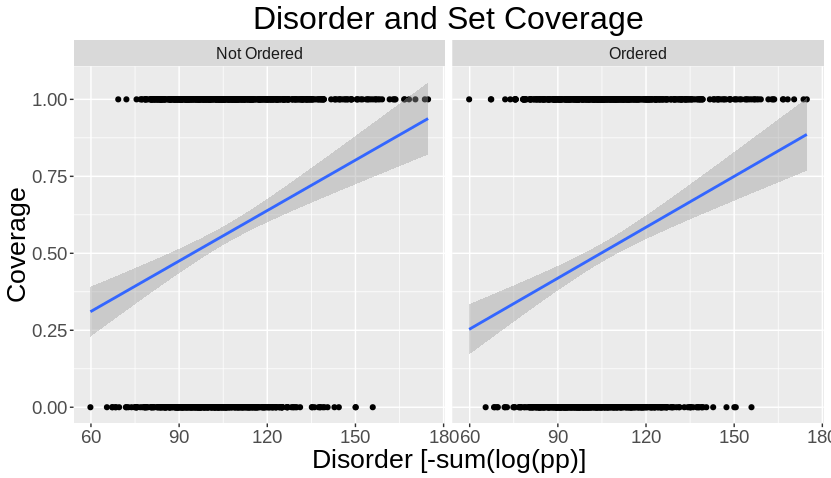
\includegraphics[scale=0.5]{images/Coverage_and_Disorder_Charts/Cov_100_sim.png}
\caption{Coverage and Disorder in  100 Simulations}
\label{100_sim}
\end{figure}




\begin{figure}[H]
\centering
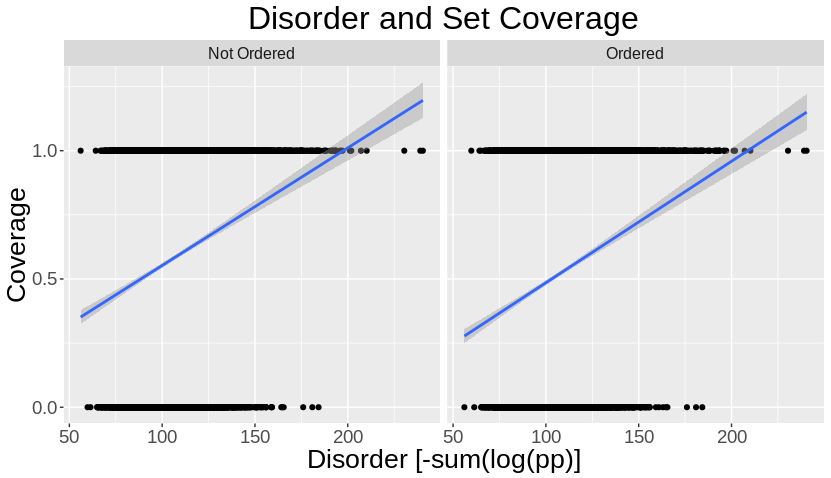
\includegraphics[scale=0.5]{images/Coverage_and_Disorder_Charts/Cov_1000_sim.png}
\caption{Coverage and Disorder in  1000 Simulations}
\label{1000_sim}
\end{figure}
